\documentclass[tikz, preview]{standalone}
\usepackage{amsfonts, amsthm, amssymb, amsmath, stmaryrd, etoolbox}
\usepackage{tikz}
\usetikzlibrary{matrix,arrows}
\newcommand{\id}{\text{id}}
\begin{document}
%%%%%%%%%%%%%%%%%	
%%%%%%%%%%%%%%%%%
\[
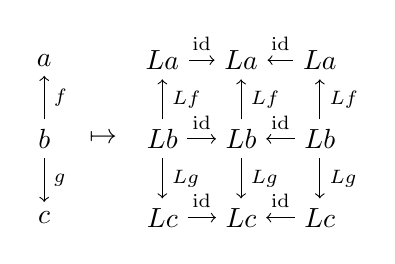
\begin{tikzpicture}
%	\draw [help lines, step=0.5, color=blue!10] (-5,-5) grid (5,5); % grid
	%
	\begin{scope}
	\node (a) at (0,1) {$ a $};
	\node (b) at (0,0) {$ b $};
	\node (c) at (0,-1) {$ c $};
	\draw [->] (b) to node [right] {\scriptsize $ f $} (a);
	\draw [->] (b) to node [right] {\scriptsize $ g $} (c);
	\end{scope}
	%
	\begin{scope}[shift={(0.75,0)}]
	\node at (0,0) {$ \mapsto $};
	\end{scope}
	%
	\begin{scope}[shift={(2.5,0)}]
	\node (ul) at (-1,1) {$ La $};
	\node (um) at (0,1) {$ La $};
	\node (ur) at (1,1) {$ La $};
	\node (ml) at (-1,0) {$ Lb $};
	\node (mm) at (0,0) {$ Lb $};
	\node (mr) at (1,0) {$ Lb $};
	\node (bl) at (-1,-1) {$ Lc $};
	\node (bm) at (0,-1) {$ Lc $};
	\node (br) at (1,-1) {$ Lc $};
	\draw [->] (ul) to node [above] {\scriptsize $ \id $} (um);
	\draw [->] (ml) to node [above] {\scriptsize $ \id $} (mm);
	\draw [->] (bl) to node [above] {\scriptsize $ \id $} (bm);
	\draw [->] (ur) to node [above] {\scriptsize $ \id $} (um);
	\draw [->] (mr) to node [above] {\scriptsize $ \id $} (mm);
	\draw [->] (br) to node [above] {\scriptsize $ \id $} (bm);
	\draw [->] (ml) to node [right] {\scriptsize $ Lf $} (ul);
	\draw [->] (ml) to node [right] {\scriptsize $ Lg $} (bl);
	\draw [->] (mm) to node [right] {\scriptsize $ Lf $} (um);
	\draw [->] (mm) to node [right] {\scriptsize $ Lg $} (bm);
	\draw [->] (mr) to node [right] {\scriptsize $ Lf $} (ur);
	\draw [->] (mr) to node [right] {\scriptsize $ Lg $} (br);
	\end{scope}
\end{tikzpicture}
\]
%%%%%%%%%%%%%%%%%
%%%%%%%%%%%%%%%%%
\end{document}
